\documentclass{llncs}

\usepackage{listings}
\usepackage{proof}
\usepackage{amssymb}
\usepackage[margin=.9in]{geometry}
\usepackage{amsmath}
\usepackage[english]{babel}
\usepackage[utf8]{inputenc}
\usepackage{enumitem}
\usepackage{filecontents}
\usepackage{calc}
\usepackage[linewidth=0.5pt]{mdframed}
\usepackage{changepage}
\usepackage{mathtools}
\usepackage{graphicx}

\allowdisplaybreaks

\usepackage{fancyhdr}
\renewcommand{\headrulewidth}{0pt}
\pagestyle{fancy}
 \fancyhf{}
\rhead{\thepage}

\lstset{tabsize=3, basicstyle=\ttfamily\small, commentstyle=\itshape\rmfamily, numbers=left, numberstyle=\tiny, language=java,moredelim=[il][\sffamily]{?},mathescape=true,showspaces=false,showstringspaces=false,columns=fullflexible,xleftmargin=5pt,escapeinside={(@}{@)}, morekeywords=[1]{objtype,module,import,let,in,fn,var,type,rec,fold,unfold,letrec,alloc,ref,application,policy,external,component,connects,to,meth,val,where,return,group,by,within,count,connect,with,attr,html,head,title,style,body,div,keyword,unit,def}}
\lstloadlanguages{Java,VBScript,XML,HTML}

\newcommand{\keywadj}[1]{\mathtt{#1}}
\newcommand{\keyw}[1]{\keywadj{#1}~}

\newcommand{\kw}[1]{\keyw{ #1 }}
\newcommand{\kwa}[1]{\keywadj{ #1 }}
\newcommand{\reftt}{\mathtt{ref}~}
\newcommand{\Reftt}{\mathtt{Ref}~}
\newcommand{\inttt}{\mathtt{int}~}
\newcommand{\Inttt}{\mathtt{Int}~}
\newcommand{\stepsto}{\leadsto}
\newcommand{\todo}[1]{\textbf{[#1]}}
\newcommand{\intuition}[1]{#1}
\newcommand{\hyphen}{\hbox{-}}

%\newcommand{\intuition}[1]{}

\newlist{pcases}{enumerate}{1}
\setlist[pcases]{
  label=\fbox{\textit{Case}}\protect\thiscase\textit{:}~,
  ref=\arabic*,
  align=left,
  labelsep=0pt,
  leftmargin=0pt,
  labelwidth=0pt,
  parsep=0pt
}
\newcommand{\pcase}[1][]{

  \if\relax\detokenize{#1}\relax
    \def\thiscase{}
  \else
    \def\thiscase{~\fbox{#1:}}
  \fi
  \item
}

\newcommand{\thm}[3]{
	\begin{large}
		\bf{#1}
	\end{large} \\\\
	\fbox{Statement.} ~ #2
	\fbox{Proof.}~ #3 \qed
}

\newcommand{\proofcase}[2]{
	\begin{adjustwidth}{1.5em}{0pt}
		\fbox{Case.}~~#1. \\ ~#2
	\end{adjustwidth}
}

\newcommand{\subcase}[1] {
	\begin{adjustwidth}{2.2em}{0pt}
		\underline{Subcase.} #1
	\end{adjustwidth}
}

\newcommand{\stmt}[1] {

\begin{adjustwidth}{2.5em}{0pt}
	#1
\end{adjustwidth}

}
\newcommand{\type}[2]{
	#1~\keyw{with} #2
}

\newcommand{\unit}[0]{ \kwa{unit} }

\newcommand{\Unit}[0]{ \kwa{Unit} }

\newcommand{\fx}[1]{ \kwa{effects}(#1) }

\newcommand{\hofx}[1]{ \kwa{ho \hyphen effects}(#1) }

\newcommand{\safe}[2]{ \kwa{safe}(#1, #2) }

\newcommand{\hosafe}[2]{ \kwa{ho \hyphen safe}(#1, #2) }

\newcommand{\arr}[3]{
	#1 \rightarrow_{#3} #2
}

\newcommand{\newd}[0]{
	\keywadj{new}_d~x \Rightarrow \overline{d = e}
}

\newcommand{\newsig}[0]{
	\keywadj{new}_\sigma~x \Rightarrow \overline{\sigma = e}
}

\newcommand{\import}[4]{
	\keywadj{import}(#1)~#2 = #3~\kw{in} #4
}

\newcommand{\annot}[2]{
	\keywadj{annot}(#1, #2)
}

\newcommand{\erase}[1]{
	\keywadj{erase}(#1)
}

\newcommand{\poly}[2]{
	\forall #1. #2
}

\newcommand{\polycap}[3]{
	\forall #1. #2~ \kw{caps} #3
}

\newcommand\defn{\mathrel{\overset{\makebox[0pt]{\mbox{\normalfont\tiny\sffamily def}}}{=}}}


\begin{document}











\section{Basic Effect Polymorphism}

\subsection*{Pseudo-Wyvern}
\begin{lstlisting}
def polymorphicWriter(x: T <: {File, Socket}): Unit with T.write =
    x.write
 
/* below invocation should typecheck with File.write as its only effect */
polymorphicWriter File
    
\end{lstlisting}

\subsection*{$\lambda$-Calculus}
\begin{lstlisting}
let pw = $\lambda \phi \subseteq$ {File.write, Socket.write}.
   $\lambda$f: Unit $\rightarrow_{\phi}$ Unit.
      f unit

in let makeWriter = $\lambda$r: {File, Socket}.
   $\lambda$x: Unit. r.write

in (pw {File.write}) (makeWriter File)
\end{lstlisting}


\subsection*{Typing}

To type the definition of $\kwa{polymorphicWriter}$:
\begin{enumerate}
	\item By \textsc{$\varepsilon$-App}\\ $\phi \subseteq \{ \kwa{F.w, S.w} \}$, x: $\Unit \rightarrow_{\phi} \Unit \vdash x~\unit: \Unit~\kw{with} \phi$.
	\item By \textsc{$\varepsilon$-Abs}\\ $\phi \subseteq \{ \kwa{F.w, S.w} \} \vdash \lambda x: \Unit \rightarrow_{\phi} \Unit. x~\unit: (\Unit \rightarrow_{\phi} \Unit) \rightarrow_{\phi} \Unit~\kw{with} \varnothing$
	\item By \textsc{$\varepsilon$-PolyFxAbs}, \\ $\vdash \forall \phi \subseteq \{ \kwa{S.w, F.w} \}. \lambda x: \Unit \rightarrow_{\phi} \Unit. x~\unit:\polycap{\phi \subseteq \{ \kwa{F.w, S.w} \}}{(\Unit \rightarrow_{\phi} \Unit) \rightarrow_{\phi} \Unit}{\varnothing}~\kw{with} \varnothing$
\end{enumerate}

\noindent
Then $\kwa{(pw~\{ File.write \})}$ can be typed as such:

\begin{enumerate}
  \setcounter{enumi}{3}
  \item By \textsc{$\varepsilon$-PolyFxApp}, \\ $\vdash \kwa{pw~\{ F.w \}}: [\{ \kwa{F.w} \}/\phi]( (\Unit \rightarrow_{\phi} \Unit) \rightarrow_{\phi} \Unit) ~\kw{with} [\{ \kwa{F.w} \}/\phi]\varnothing \cup \varnothing$
\end{enumerate}

\noindent
The judgement can be simplified to:

\begin{enumerate}
	\setcounter{enumi}{4}
	\item $\vdash \kwa{pw~\{ F.w \}}: (\Unit \rightarrow_{\{\kwa{F.w}\}} \Unit) \rightarrow_{\{\kwa{F.w}\}} \Unit ~\kw{with} \varnothing$
\end{enumerate}

\noindent
Any application of this function, as in $\kwa{(pw~\{File.write\}) (makeWriter~ File)}$, will therefore type as having the single effect $\kwa{F.w}$ by applying \textsc{$\varepsilon$-App} to judgement (5).




























\section{Dependency Injection}

\subsection*{Pseudo-Wyvern}

An HTTPServer module provides a single $\kwa{init}$ method which returns a $\kwa{Server}$ that responds to HTTP requests on the supplied socket.
\begin{lstlisting}
module HTTPServer

def init(out: A <: {File, Socket}): $\kwa{Str}\rightarrow_{A.write}\Unit$ with $\varnothing$ =
   $\lambda$ msg: Str.
      if (msg == ``POST'') then out.write(``post response'')
      else if (msg == ``GET'') then out.write(``get response'')
      else out.write(``client error 400'')
\end{lstlisting}

\noindent
The main module calls $\kwa{HTTPServer.init}$ with the $\kwa{Socket}$ it should be writing to.

\begin{lstlisting}
module Main
require HTTPServer, Socket

def main(): Unit =
   HTTPServer.init(Socket) ``GET /index.html''
\end{lstlisting}

\noindent
The testing module calls $\kwa{HTTPServer.init}$ with a $\kwa{LogFile}$, perhaps so the responses of the server can be tested offline.

\begin{lstlisting}
module Testing
require HTTPServer, LogFile

def testSocket():  =
   HTTPServer.init(LogFile) ``GET /index.html''
\end{lstlisting}


\subsection*{$\lambda$-Calculus}

\noindent
The HTTPServer module:
\begin{lstlisting}
MakeHTTPServer = $\lambda$x: Unit.
   $\lambda \phi \subseteq \{ \kwa{LogFile.write, Socket.write} \}$.
      $\lambda$f: Str $\rightarrow_{\phi}$ Unit.
         $\lambda$msg: Str.
            f msg
\end{lstlisting}

\noindent
The Main module:

\begin{lstlisting}
MakeMain = $\lambda$hs: HTTPServer. $\lambda$sock: {Socket}.
   $\lambda$x: Unit.
      let socketWriter = ($\lambda$s: {Socket}. $\lambda$x: Unit. s.write) sock in
      let theServer = hs {Socket.write} socketWriter in
      theServer ``GET/index.html''
\end{lstlisting}

\noindent
The Testing module:

\begin{lstlisting}
MakeTest = $\lambda$hs: HTTPserver. $\lambda$lf: {LogFile}.
   $\lambda$x: Unit.
      let logFileWriter = ($\lambda$l: {LogFile}. $\lambda$x: Unit. l.write) lf in
      let theServer = hs {LogFile.write} logFileWriter in
      theServer ``GET/index.html''
\end{lstlisting}

\noindent
A single, desugared program for production would be:

\begin{lstlisting}
let MakeHTTPServer = $\lambda$x: Unit.
   $\lambda \phi \subseteq \{ \kwa{LogFile.write, Socket.write} \}$.
      $\lambda$f: Str $\rightarrow_{\phi}$ Unit.
         $\lambda$msg: Str.
            f msg

in let Run = $\lambda$Socket: {Socket}.
   let HTTPServer = MakeHTTPServer unit in
   let Main = MakeMain HTTPServer Socket in
   Main unit

in Run Socket 
\end{lstlisting}

\noindent
A single, desugared program for testing would be:

\begin{lstlisting}
let MakeHTTPServer = $\lambda$x: Unit.
   $\lambda \phi \subseteq \{ \kwa{LogFile.write, Socket.write} \}$.
      $\lambda$f: Str $\rightarrow_{\phi}$ Unit.
         $\lambda$msg: Str.
            f msg

in let Run = $\lambda$LogFile: {LogFile}.
   let HTTPServer = MakeHTTPServer unit in
   let Main = MakeMain HTTPServer LogFile in
   Main unit

in Run LogFile
\end{lstlisting}

\noindent
Note how the HTTPServer code is identical in the testing and production examples.

\subsection*{Typing}


\begin{lstlisting}
let MakeHTTPServer = $\lambda$x: Unit.
   $\lambda \phi \subseteq \{ \kwa{LogFile.write, Socket.write} \}$.
      $\lambda$f: Str $\rightarrow_{\phi}$ Unit.
         $\lambda$msg: Str.
            f msg
\end{lstlisting}

\noindent
To type $\kwa{MakeHTTPServer}$:

\begin{enumerate}
	\item By \textsc{$\varepsilon$-App}, \\
	$\kwa{x: Unit,~ \phi \subseteq \{LF.w, S.w\}, f: Str \rightarrow_{\phi} Unit,~ msg: Str}$ \\
	$\vdash \kwa{f~msg: Unit~\kw{with} \phi}$
	
	\item By \textsc{$\varepsilon$-Abs}, \\
	$\kwa{x: Unit,~ \phi \subseteq \{LF.w, S.w\}, f: Str \rightarrow_{\phi} Unit}$ \\
	$\vdash \kwa{\lambda msg: Str.~f~msg: Str \rightarrow_{\phi} Unit~\kw{with} \varnothing }$

	\item By \textsc{$\varepsilon$-Abs}, \\
	$\kwa{x: Unit,~ \phi \subseteq \{LF.w, S.w\}}$ \\
	$\vdash \kwa{\lambda f: Str \rightarrow_{\phi} Unit.~\lambda msg: Str.~f~msg:}\\
	\kwa{ (Str \rightarrow_{\phi} Unit) \rightarrow_{\varnothing} (Str \rightarrow_{\phi} Unit)~\kw{with} \varnothing }$

	\item By \textsc{$\varepsilon$-PolyFxAbs}, \\
	$\kwa{x: Unit}$ \\
	$\vdash \kwa{\lambda \phi \subseteq \{ LF.w, S.w \}.~ \lambda f: Str \rightarrow_{\phi} Unit.~\lambda msg: Str.~f~msg:}$\\
	$\kwa{\polycap{\phi \subseteq \{ LF.w, S.w\}}{(Str \rightarrow_{\phi} Unit) \rightarrow_{\varnothing} (Str \rightarrow_{\phi} Unit)}{\varnothing}~\kw{with} \varnothing}$

	\item By \textsc{$\varepsilon$-Abs}, \\
	$\vdash \kwa{\lambda x: Unit. ~\lambda \phi \subseteq \{ LF.w, S.w \}.~ \lambda f: Str \rightarrow_{\phi} Unit.~\lambda msg: Str.~f~msg:}$\\
	$\kwa{Unit} \rightarrow_{\varnothing} \kwa{\polycap{\phi \subseteq \{ LF.w, S.w\}}{(Str \rightarrow_{\phi} Unit) \rightarrow_{\varnothing} (Str \rightarrow_{\phi} Unit)}{\varnothing}~\kw{with} \varnothing}$
\end{enumerate}

\noindent
Note that after two applications of $\kwa{MakeHTTPServer}$, as in $\kwa{MakeHTTPServer~unit~\{Socket.write\}}$, it would type as follows:

\begin{enumerate}
	\setcounter{enumi}{5}
	\item By \textsc{$\varepsilon$-PolyFxApp}, \\
	$\kwa{x: Unit}$\\
	$\kwa{\vdash MakeHTTPServer~unit~\{S.w\}:}$\\
	$\kwa{(Str \rightarrow_{\{S.w\}} Unit) \rightarrow_{\varnothing} (Str \rightarrow_{\{S.w\}} Unit)~\kw{with} \varnothing}$
\end{enumerate}

\noindent
After fixing the polymorphic set of effects, possessing this function only gives you access to the $\kwa{Socket.write}$ effect.













\section{Map Function}

\subsection*{Pseudo-Wyvern}
\begin{lstlisting}
def map(f: A $\rightarrow_{\phi}$ B, l: List[A]): List[B] with $\phi$ =
	if isnil l then []
	else cons (f (head l)) (map (tail l f))
\end{lstlisting}

\subsection*{$\lambda$-Calculus}
\begin{lstlisting}
map = $\lambda \phi$. $\lambda$A. $\lambda$B.
  $\lambda$f: A$\rightarrow_{\phi}$B.
    (fix ($\lambda$map: List[A] $\rightarrow$ List[B]).
      $\lambda$l: List[A].
        if isnil l then []
        else cons (f (head l)) (map (tail l f)))
\end{lstlisting}

\subsection*{Typing}

\begin{itemize}
	\item This has the type: $\forall \phi. \forall A. \forall B. (A \rightarrow_{\phi} B)  \rightarrow_{\varnothing} \kwa{List}[A] \rightarrow_{\phi} \kwa{List}[B]~ \kw{with} \varnothing$.
	\item $\kwa{map}~\varnothing$ is a pure version of map.
	\item $\kwa{map}~\{ \kwa{File.*} \}$ is a version of map which can perform operations on $\kwa{File}$.
\end{itemize}



\section{Imports Are an Upper Bound on Polymorphic Capabilities}

\subsection{Example 1}

\begin{lstlisting}
let polywriter = $\lambda \phi \subseteq \{ \kwa{File.write, Socket.write} \}$. $\lambda$f: Unit $\rightarrow_{\phi}$ Unit. f unit

import({File.*}) 
   pw = polywriter
   f = File
in
   e
\end{lstlisting}

\noindent
In the unannotated code $e$, you can never make $\kwa{pw}$ return a socket-writing function, because there is no socket-writing capability in scope that it could be given. However, this example should fail for a different reason: there is a file capability in scope, and you could pass $\kwa{pw}$ a function which captures any effect on that file, which would violate its signature. For instance:

\begin{lstlisting}
import({File.*}) 
   pw = polywriter
   f = File
in
   pw {File.write} ($\lambda$x: Unit. f.read)
\end{lstlisting}

\noindent
\textbf{This example should typecheck, since typechecking of the unannotated body strips all annotations from the imported capabilities. However, as of 17/05/2017, there is no way to apply effect-polymorphic types in an unannotated context.}\\

\subsection*{Derivation}

For this section we are going to be conflating the name of a variable with its type (so $pw$ really means the type of the variable $pw$, which is the effect-polymorphic type). Firstly, note that $\fx{pw} = \hofx{pw} = \{ \kwa{File.write, Socket.write} \}$. Then: \\

\noindent
 $\kwa{effects}(pw, \{ \{ \kwa{File} \} \})\\
=  \fx{pw} \cap \fx{\{\kwa{File}\}}\\
=  \{ \kwa{File.write, Socket.write} \} \cap \{ \kwa{File.*} \}\\
=  \{ \kwa{File.write} \} \subseteq \varepsilon_s = \{ \kwa{File.*} \}$\\

\noindent
And also: \\

\noindent
$\kwa{effects}(\{ \kwa{File} \}, \{ pw \})\\
= \fx{\{ \kwa{File} \}}\\
=\{ \kwa{File.*} \} \subseteq \varepsilon_s = \{ \kwa{File.*} \}$\\

\noindent
However, $\hosafe{pw, \varepsilon_s}$ will fail, causing this example to not typecheck. \\

\noindent
$\hosafe{pw}{\varepsilon_s}\\
= \hosafe{ \polycap{\phi \subseteq \{ \kwa{File.write, Socket.write} \}}{((\Unit \rightarrow_{\phi} \Unit) \rightarrow_{\phi} \Unit)}{\varnothing}}{\{ \kwa{File.*} \}}\\
= \varnothing \subseteq \{ \kwa{File.*} \} \land \safe{((\Unit \rightarrow_{\{F.w, S.w\}} \Unit) \rightarrow_{\{  F.w, S.w \}} \Unit)}{\{\kwa{File.*}\}}\\
= \{ \kwa{File.*} \} \subseteq \{ \kwa{File.write, Socket.write} \} \land ......$\\

\noindent 
The last line is not true, because $\{ \kwa{File.*} \} \subseteq \{ \kwa{File.write, Socket.write} \}$ is not true. The inutition here is that it is failing because you might pass some capability into $pw$ which does any file operation --- and $pw$ only permits it to be writing.


\subsection{Example 2}

This is a modified version of the above example. Instead of passing in a $\kwa{File}$, we pass in a restricted capability that only endows its bearer with write operations on a $\kwa{File}$. This modified version should safely typecheck. The point is that, although the polymorphic function could theoretically be applied so that it returns a socket-writing function, this can't be done in practice because no socket-writing capability can be given to it. It's therefore safe to leave $\kwa{Socket.write}$ out of the selected authority.

\begin{lstlisting}
let polywriter = $\lambda \phi \subseteq \{ \kwa{File.write, Socket.write} \}$. $\lambda$f: Unit $\rightarrow_{\phi}$ Unit. f unit

let fwriter = $\lambda$x: Unit. File.write

import({File.write}) 
   pw = polywriter
   fw = fwriter
in
   pw {File.write} fw
\end{lstlisting}

\noindent
Now we can verify that it meets the conditions of \textsc{$\varepsilon$-Import}. Firstly, note that $\fx{pw} = \hofx{pw} = \{ \kwa{File.write, Socket.write} \}$, and $\fx{fw} = \{ \kwa{File.write} \}$ and $\hofx{fw} = \varnothing$.\\

\noindent
$\kwa{effects}(pw, \{ fw \})\\
= \fx{pw} \cap \fx{fw}\\
= \{ \kwa{File.write, Socket.write} \} \cap \{ \kwa{File.write} \}\\
= \{ \kwa{File.write} \} \subset \varepsilon_s = \{ \kwa{File.write} \}$\\

\noindent
And also\\

\noindent
$\kwa{effects}(fw, \{ pw \})\\
= \fx{fw}\\
= \{ \kwa{File.write} \} \subseteq \varepsilon_s = \{ \kwa{File.write} \}$\\

\noindent
Next we shall check that $\hosafe{pw}{\varepsilon_s}$ and $\hosafe{fw}{\varepsilon_s}$.\\

\noindent
$\hosafe{pw}{\varepsilon_s}\\
=\hosafe{ \polycap{\phi \subseteq \{ \kwa{File.write, Socket.write} \}}{((\Unit \rightarrow_{\phi} \Unit) \rightarrow_{\phi} \Unit)}{\varnothing}}{\{ \kwa{File.write} \}}\\
=\varnothing \subseteq \{ \kwa{File.write} \} \land \safe{((\Unit \rightarrow_{\{ \kwa{F.w, S.w} \}} \Unit) \rightarrow_{\{ \kwa{F.w, S.w} \}} \Unit)}{\{ \kwa{File.write} \}}\\
=\safe{((\Unit \rightarrow_{\{ \kwa{F.w, S.w} \}} \Unit) \rightarrow_{\{ \kwa{F.w, S.w} \}} \Unit)}{\{ \kwa{File.write} \}}\\
= \{ \kwa{File.write} \} \subseteq \{ \kwa{File.write, Socket.write} \} \land \hosafe{\Unit \rightarrow_{\{ \kwa{F.w, S.w} \}} \Unit }{\{ \kwa{File.write} \}} \land \safe{\Unit}{\{ \kwa{File.write} \}}\\
= \hosafe{\Unit \rightarrow_{\{ \kwa{F.w, S.w} \}} \Unit }{\{ \kwa{File.write} \}}\\
= \safe{\Unit}{\{ \kwa{F.w, S.w} \}}\\
= \kwa{true}$\\

\noindent
$\hosafe{fw}{\varepsilon_s}\\
= \hosafe{\Unit \rightarrow_{\{\kwa{File.write}\}} \Unit}{\{ \kwa{File.write} \}}\\
= \safe{\Unit}{\{ \kwa{File.write} \}} \land \hosafe{\Unit}{\{ \kwa{File.write} \}}\\
= \kwa{true}$

\noindent
So it successfully accepts.

\section{Violating a polymorphic function that has been fixed}

Malicious code tries to import polywriter, where the effect-set has been fixed to $\{ \kwa{File.write} \}$, and then calls it with $\kwa{ \{Socket.write\} }$. The example should reject.

\begin{lstlisting}

let polywriter = $\lambda \phi \subseteq \{ \kwa{File.write, Socket.write} \}$. $\lambda$f: Unit $\rightarrow_{\phi}$ Unit. f unit

import({File.*, Socket.*})
   filewriter = polywriter {File.write}
   s = $\lambda$x: Unit. Socket.write
in
   filewriter s
\end{lstlisting}

Safely rejects because the higher-order safety check is not true (acknowledging that $\kwa{filewriter}$ could be passed a capability exceeding its authority). \\

$\hosafe{(\Unit \rightarrow_{\kwa{\{File.write\}}} \Unit) \rightarrow_{\kwa{\{File.write\}}} \Unit}{\kwa{ \{File.*, Socket.*\} }}$ \\

$= \safe{\Unit \rightarrow_{\kwa{\{File.write\}}} \Unit}{\{\kwa{File.*, Socket.*}\}} \land \hosafe{\Unit}{\{\kwa{File.*, Socket.*}\}}$ \\

$= \safe{\Unit \rightarrow_{\kwa{\{File.write\}}} \Unit}{\{\kwa{File.*, Socket.*}\}}$ \\

$= \{\kwa{File.*, Socket.*}\} \subseteq \{ \kwa{File.*} \}$ \\

which is false.



\section{Composing polymorphic functions (artificial example)}

\begin{lstlisting}
$\lambda \phi_1 \subseteq$ { File.write, File.read }.
   $\lambda \phi_2 \subseteq \phi_1$.
      $\lambda$f: $\Unit \rightarrow_{ \phi_1 } \Unit$.
         $\lambda$g: $\Unit \rightarrow_{ \phi_2 } \Unit$.
            let _ = f unit in g unit 
\end{lstlisting}


~\\

\section{Stress-Testing Two-Variable Version of Effects}

The intuition behind $\kwa{fx}(\hat \tau_A, \overline{\hat \tau})$ is that we are computing the possible effects of an expression of type $\hat \tau_A$, when only the capabilities in $\overline{\hat \tau}$ are in scope. For example, consider the example of a function which abstracts over any function with effects on $\kwa{File}$:

\begin{lstlisting}
let pw =
   $\lambda \phi \subseteq$ {File.*}.
      $\lambda$f: Unit $\rightarrow_{\phi}$ Unit.
         f unit
in ...
\end{lstlisting}

Consider a function which only writes to a file:

\begin{lstlisting}
let fw =
   $\lambda$x: Unit. File.write
\end{lstlisting}

Then consider the following use of an import construct:

\begin{lstlisting}
import($\varepsilon_s$)
   x$_1$ = pw, x$_2$ = fw
in e
\end{lstlisting}

What is the smallest, correct $\varepsilon_s$? A conservative answer is to say $\{ \kwa{File.*} \}$ --- indeed, $\kwa{pw}$ is allowed to have any of these effects, provided someone gives it to them. But in the context of $e$, the only effect which can be realised is $\{ \kwa{File.write} \}$, so an even better answer would be $\varepsilon_s$. This is the idea behind the two-variable version of $\kwa{effects}$ --- it attempts to give an upper-bound on the effects something can have by considering the capabilities in scope.

Some terminology: for simplicity, let $\kwa{type}(\hat e)$ be the type obtained by type-checking $\hat e$ in the smallest possible context. In most cases it should be obvious what this is.In pretty much every following example, that is going to be $\varnothing$.

\subsection{1 Poly, 1 Non-Poly}

Consider a context where only the following two capabilites are in scope:
\begin{enumerate}
	\item $\kwa{pw = \lambda \phi \subseteq \{\kwa{File.*}\}. ~\lambda f: \Unit \rightarrow_{\phi} \Unit. ~f ~\unit}$
	\item $\kwa{fw = \lambda x: Unit.~File.write}$
\end{enumerate}

\noindent
Their types are the following:

\begin{enumerate}
	\item $\kwa{\hat \tau_1 = type(pw) = \forall \phi \subseteq \{ File.* \}.~(Unit \rightarrow_{\phi} Unit) \rightarrow_{\phi} Unit~caps~\varnothing~with~\varnothing}$
	\item $\kwa{\hat \tau_2 = type(fw) = Unit \rightarrow_{\{File.write\}} Unit~with~\varnothing}$
\end{enumerate}

\noindent
Their conservative effect approximations are:

\begin{enumerate}
	\item $\kwa{effects(type(pw)) = \{File.*\} }$
	\item $\kwa{effects(type(fw)) = \{File.write\} }$
\end{enumerate}

\noindent
The two-variable version of $\kwa{effect}$ gives the following better approximation for the polymorphic type $\kwa{type(pw)}$:

\begin{enumerate}
	\item $\kwa{effects(type(pw), \{ type(fw) \}) = effects(type(pw)) \cap effects(type(fw)) = \{File.write\}}$
\end{enumerate}

\noindent
Which is a correct, tighter upper bound.

\subsection{2 Poly Imports}

The two capabilities are in scope:
\begin{enumerate}
	\item $\kwa{pw = \lambda \phi \subseteq \{\kwa{File.*}\}. ~\lambda f: \Unit \rightarrow_{\phi} \Unit. ~f ~\unit}$
	\item $\kwa{sw = \lambda \phi \subseteq \{\kwa{Socket.*}\}. ~\lambda f: \Unit \rightarrow_{\phi} \Unit. ~f ~\unit}$
\end{enumerate}

\noindent
Their types are the following:

\begin{enumerate}
	\item $\kwa{\hat \tau_1 = type(pw) = \forall \phi \subseteq \{ File.* \}.~(Unit \rightarrow_{\phi} Unit) \rightarrow_{\phi} Unit~caps~\varnothing~with~\varnothing}$
	\item $\kwa{\hat \tau_2 = type(sw) = \forall \phi \subseteq \{ Socket.* \}.~(Unit \rightarrow_{\phi} Unit) \rightarrow_{\phi} Unit~caps~\varnothing~with~\varnothing}$
\end{enumerate}

\noindent
Which have the following conservative effect approximations:

\begin{enumerate}
	\item $\kwa{effects(type(pw)) = \{File.*\} }$
	\item $\kwa{effects(type(sw)) = \{Socket.*\} }$
\end{enumerate}

\noindent
The two-variable version of $\kwa{effect}$ gives the following better approximations:

\begin{enumerate}
	\item $\kwa{effects(type(pw), \{ type(sw) \}) = effects(type(pw)) \cap effects(type(sw)) = \{ File.* \} \cap \{ Socket.* \} = \varnothing}$
	\item $\kwa{effects(type(sw), \{ type(pw) \}) = effects(type(sw)) \cap effects(type(pw)) = \{ Socket.* \} \cap \{ File.* \} = \varnothing}$
\end{enumerate}

\noindent
These upper bounds are tighter. They are also correct --- no matter how you fix $\kwa{pw}$ or $\kwa{sw}$, there is no way to pass one to the other in order to invoke an effect.

\subsection{1 Poly, 1 Unusable Non-Poly}

\noindent
The following two capabilities are in scope. This time, $\kwa{fw}$ writes to both $\kwa{File}$ and $\kwa{Socket}$.

\begin{enumerate}
	\item $\kwa{pw = \lambda \phi \subseteq \{\kwa{File.*}\}. ~\lambda f: \Unit \rightarrow_{\phi} \Unit. ~f ~\unit}$
	\item $\kwa{fw = \lambda x: Unit.~File.write;~Socket.write}$
\end{enumerate}

\noindent
Their types are the following:

\begin{enumerate}
	\item $\kwa{\hat \tau_1 = type(pw) = \forall \phi \subseteq \{ File.* \}.~(Unit \rightarrow_{\phi} Unit) \rightarrow_{\phi} Unit~caps~\varnothing~with~\varnothing}$
	\item $\kwa{\hat \tau_2 = type(fw) = Unit \rightarrow_{\{File.write, Socket.write\}} Unit~with~\varnothing}$
\end{enumerate}

\noindent
Their conservative effect approximations are:

\begin{enumerate}
	\item $\kwa{effects(type(pw)) = \{File.*\} }$
	\item $\kwa{effects(type(fw)) = \{File.write, Socket.write\} }$
\end{enumerate}

\noindent
The two-variable version of $\kwa{effects}$ will give the following approximation for $\kwa{type(pw)}$:

\begin{enumerate}
	\item $\kwa{effects(type(pw), \{ type(fw) \}) = \{File.*\} \cap \{File.write, Socket.write\} = \{File.write\}}$
\end{enumerate}

\noindent
This is a better approximation than $\kwa{File.*}$, but it's still not a tight approximation. The tight approximation in this situation is $\varnothing$, because you can never pass $\kwa{fw}$ to any instantiation of $\kwa{pw}$ --- any instantiation of $\kwa{pw}$ can only be passed a function with effects on $\kwa{File}$, but $\kwa{fw}$ has effects on $\kwa{Socket}$. The issue: we only intersect the polymorphic effects with the effects of a capability in scope if that capability's effects are contained in the upper-bound of the polymorphic effects. If not, the maximal set of effects that could be incurred with that capability is $\varnothing$, because it can't be passed to the polymorphic code. The following diagram illustrates:


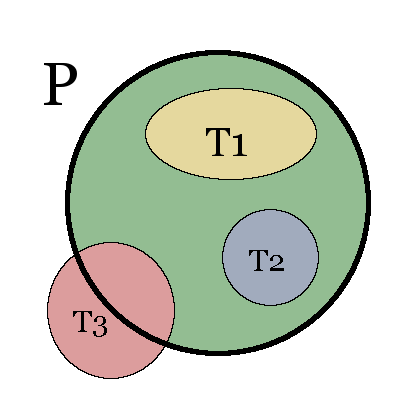
\includegraphics{effects}

The circles represent the effects of the labelled types. So the green circle is $\kwa{effects}(P)$. We currently approximate $\kwa{effects}(p, \{ T_1, T_2, T_3\})$ as $\kwa{effects}(p) \cap (\kwa{effects}(T_1) \cup \kwa{effects}(T_2) \cup \kwa{effects}(T_3))$. This approximation includes those effects in both $\fx{P} \cap \fx{T_3}$ --- but these effects can't ever be used by $p$, since the capability $T_3$ contains more effects than stipulated by the upper-bound of $p$. Therefore we want to exclude $T_3$ from our union, and instead give the approximation as $\kwa{effects}(p) \cap (\kwa{effects}(T_1) \cup \kwa{effects}(T_2))$. That is, we want to exclude $\fx{T_3}$ from our approximation because it contains effects outside of $\fx{P}$.

Here are two proposed amendments to $\kwa{effects}(p, \overline{\hat \tau})$:

\begin{enumerate}

	\item Have two cases based on whether $\kwa{effects}(\hat \tau_i) \subseteq \kwa{effects}(p)$. They might look like the following

  \begin{equation*}
    \kwa{effects}(p, \{\hat \tau_i\})  = \bigcup_{i}
    \begin{cases*}
      \fx{\hat \tau_i} \cap \fx{p}        & if $\fx{\hat \tau_i} \subseteq \fx{P}$ \\
      \varnothing & otherwise
    \end{cases*}
  \end{equation*}

	\item Notice that the result is always going to be a subset of $\kwa{effects}(p)$ (either $\varnothing$ or the intersection of $\kwa{effects}(p)$ with the effects of some capability in scope).
	
   \begin{equation*}
    \kwa{effects}(p, \{\hat \tau_i\})  = \bigcup[\mathcal{P}(p) \cap \bigcup_{i} \{\fx{\hat \tau_i}\}]
  \end{equation*}
  
Now if there is a capability in $\fx{\hat \tau_i} \setminus \fx{p}$ then $\{ \fx{\hat \tau_i} \}$ won't be in $\mathcal{P}(p)$, so the result will be $\varnothing$.
  
\end{enumerate}

%\section{Accessing Database via Expert}

\subsection{Instantiate 1 Poly and Pass To Another Poly}

Consider the following capabilities:

\begin{lstlisting}
pw = $\lambda \phi \subseteq$ {File.*, Socket.*}.
        $\lambda$f: Unit $\rightarrow_{\phi}$ Unit. f unit

pa = $\lambda \phi \subseteq$ {File.*}.
        $\lambda$f: Unit $\rightarrow_{\phi}$ Unit.
           let _ = Socket.write in f unit

fw = $\lambda$x: Unit. File.write
\end{lstlisting}

\noindent
Note how $\kwa{pa}$, when fixed with an effect-set, will ask for a function with those effects and then instrument it with the $\kwa{Socket.write}$ effect.

The maximal set of effects that can be achieved with these capabilities is $\{ File.write, Socket.write \}$, in the following way:

\begin{lstlisting}
import({File.write, Socket.write})
   pw = pw, fw = fw, pa = pa
in
   let pw2 = pw {File.write, Socket.write} in
   let pa2 = pw {File.write} in
   pw2 (pa2 fw) /* incurs File.write, Socket.write */
\end{lstlisting}

\noindent
Their types are the following:

\begin{enumerate}
	\item $\kwa{type(pw) = \forall \phi \subseteq \{ File.*, Socket.* \}.~(Unit \rightarrow_{\phi} Unit) \rightarrow_{\phi} Unit~caps~\varnothing~with~\varnothing}$ 
	\item $\kwa{type(pa) = \forall \phi \subseteq \{ File.* \}.~(Unit \rightarrow_{\phi} Unit) \rightarrow_{\varnothing} (Unit \rightarrow_{\phi \cup \{Socket.write\}} Unit)}$
	\item $\kwa{type(fw) = Unit \rightarrow_{\{File.write\}} Unit~with~\varnothing}$
\end{enumerate}

\noindent
Their conservative effect approximations are:

\begin{enumerate}
	\item $\kwa{effects(type(pw)) = \{File.*, Socket.* \} }$
	\item $\kwa{effects(type(pa)) = \{File.*, Socket.write \}}$
	\item $\kwa{effects(type(fw)) = \{File.write\} }$
\end{enumerate}

\noindent
If we use the two-variable version of $\kwa{effects}$ to approximate $\kwa{pa}$, then we get the following:

\begin{enumerate}
	\item $\kwa{effects(type(pw), \{type(pa), type(fw)\}) = \{ File.*, Socket.write \}}$
\end{enumerate}

\noindent
Which is correct. It also doesn't matter whether you use the old version of $\kwa{effects}$ or the updated version from the previous section; they give the same answer. However, if you try to apply the two-variable version of $\kwa{effects}$ to approximate $\kwa{pw}$ you get:

\begin{enumerate}
	\setcounter{enumi}{1}
	\item $\kwa{effects(type(pw), \{type(pa), type(fw)\}) = \{File.*, Socket.write\}}$
\end{enumerate}

Which is correct, but not a tight upper-bound. Both versions of $\kwa{effects}$ give this answer. The problem arises from when you intersect the (conservative) effects of $\kwa{pw}$ with the (conservative) effects of $\kwa{pa}$. Both $\fx{pa}$ and $\fx{pw}$ have operations on $\kwa{File}$ which can't ever be invoked, so when their conservative approximations are intersected, we get every operation on $\kwa{File}$ in the result.

\subsection{Pass Uninstantiated Poly To Another Poly}

Consider the following capabilities:

\begin{lstlisting}
/* A polymorphic id function over a type A, which incurs an effect $\phi_1$ before returning the input argument */
pid = $\lambda \Phi_1. \lambda A.$
   $\lambda$f: Unit$\rightarrow_{\Phi_1}$Unit.
      $\lambda$a: A. let _ = f unit in a

/* A polymorphic function which takes a polymorphic abstraction $P$ and wraps it in a computation $f$ with effect $\Phi_3$ */
pp = $\lambda$P <: $\forall \Phi_2. \forall A. (\Unit \rightarrow_{\Phi_2} \Unit) \rightarrow_{\varnothing} A \rightarrow_{\Phi_2} A$
   $\lambda \Phi_3$. $\lambda f: \Unit \rightarrow_{\Phi_3} \Unit$. $\lambda p: P$.
      let _ = f unit in p

/* Capabilities which capture the write operation on File and Socket */
fw = $\lambda$x:Unit. File.write
sw = $\lambda$x:Unit. Socket.write
\end{lstlisting}

\noindent
They have the following conservative effect approximations:

\begin{enumerate}
	\item $\fx{pp} = \fx{pid} = R \times \Pi$
	\item $\fx{fw} = \{\kwa{File.write}\}$
	\item $\fx{sw} = \{\kwa{Socket.write}\}$
\end{enumerate}

\noindent
The naive definition does not give a better approximation. For example,\\

\noindent
$\kwa{effects}(pid, {pp, fw, sw}) =$ \\
$(\fx{pid} \cap \fx{pp}) \cup (\fx{pid} \cap \fx{fw}) \cup (\fx{pid} \cap \fx{sw}) = $ \\
$R \times \Pi \cup \{\kwa{File.write}\} \cup \{\kwa{Socket.write}\} =$\\
$R \times \Pi$



\subsection{Regular Function Returns Poly}

Consider the following capabilities:

\begin{lstlisting}
fw = $\lambda$x: Unit. File.write

sw = $\lambda$x: Unit. Socket.write

pw = $\lambda \Phi \subseteq$ {File.*, Socket.*}.
         $\lambda$f: Unit $\rightarrow_{\Phi}$ Unit. f unit

g = $\lambda$x: Unit. pw
\end{lstlisting}

\noindent
Now consider the following $\kwa{import}$ expression, which only imports $\kwa{fw}$, $\kwa{sw}$, and $\kwa{g}$.

\begin{lstlisting}
import({File.write, Socket.write})
   fw = fw, sw = sw, g = g
in ...
\end{lstlisting}

\noindent
The types are the following:

\begin{enumerate}
   \item $\kwa{type(fw)} = \Unit \rightarrow_{\kwa{\{File.write\}}} \Unit$
   \item $\kwa{type(sw)} = \Unit \rightarrow_{\kwa{\{Socket.write\}}} \Unit$
   \item $\kwa{type(pw)} = \lambda \Phi \subseteq \kwa{\{File.*, Socket.*\}}. (\Unit \rightarrow_{\Phi} \Unit) \rightarrow_{\Phi} \Unit$
   \item $\kwa{type(g)} = \Unit \rightarrow_{\varnothing} \kwa{type(pw)} $
\end{enumerate}

\noindent
Their conservative effects:

\begin{enumerate}
	\item $\kwa{effects(type(fw)) = \{File.write\}}$
	\item $\kwa{effects(type(sw)) = \{Socket.write\}}$
	\item $\kwa{effects(type(pw)) = \{File.*, Socket.*\}}$
	\item $\kwa{effects(type(g)) = \{File.*, Socket.*\}}$
\end{enumerate}

\noindent
Note that since $g$ is not polymorphic, any of the approximations of its effects so far will give $\{ \kwa{File.*, Socket.*} \}$.









\end{document}





